\documentclass[a4paper,10pt]{article}
%\documentclass[preview=false]{standalone}
% %%%% Define new conditional \ifplastex
% %%%% This ensure that the file complied normally without plasTeX.
\usepackage{plastex}

\usepackage{hyperref}

\ifplastex\else
\usepackage{standalone} %%%% Only load standalone when not in plasTeX
\standalonetrue
\usepackage{longtable} %%%% Only load longtable and ltcaption when not in plasTeX
\usepackage{ltcaption}
\fi

% Package for typesetting URLs
\usepackage{url}

% Package for including graphics.
\usepackage{graphicx}

\usepackage{multicol}

\usepackage{bsymb}

% Package for typesetting Event-B models
\usepackage[colour]{eventB}
%\usepackage{eventB-vhdl}

% Package for typesetting dates and times
\ifplastex
\newcommand{\EMFEMFManualDate}{July 27th, 2017}
\else
\usepackage{datetime}
\newdate{EMFEMFManualDate}{27}{7}{2017}
\fi
\newcommand{\EMFEMFFeatureVersion}{2.2.1}
\newcommand{\EMFEMFManualVersion}{0.0.1}

% Title
\title{EMF2EMF Transformation Framework Developers Manual} 

% Author
\author{%s
  Colin Snook\\%
  ECS, University of Southampton\\%
  \texttt{\href{mailto:cfs@ecs.soton.ac.uk}{cfs at ecs dot soton dot ac dot uk}}%
}%


% Date
\date{%
  Version \EMFEMFManualVersion\\%
  (for feature version \EMFEMFFeatureVersion)\\
  \ifplastex
  \EMFEMFManualDate
  \else
  \displaydate{EMFEMFManualDate}%
  \fi
}

\begin{document}
\ifplastex%
\maketitle% Make title if in plasTeX mode.
\else%
 \ifstandalone%
 \maketitle % Make title if in standalone mode.
 \else%
 \fi%
\fi%

\section{EMF2EMF Translator Overview}
\label{sec:overview}

EMF2EMF is a generic framework for writing EMF to EMF model transformations in Java. Translators can be written by declaring a translator and a set of rule classes. Each rule class handles instances of a particular EMF meta-class as input. EMF2EMF provides a lightweight and efficient framework with a small footprint compared to declarative and interpretive M2M translators such as QVT, ATL or ETL. The down-side is that you have to write the details in Java instead of a nice declarative language. However, the framework structures your translation into manageable tasks to ease the task of writing your translator.


%%% Local Variables:
%%% mode: latex
%%% TeX-master: "user_manual"
%%% End:


\section{Getting Started}
\label{sec:getting-started}

\subsection{Setup}
\label{sec:setup}

\begin{itemize}
\item 
In order to start using the EMF2EMF translator you need to make the EMF2EMF translator plugin available to your code. 
You do this either by importing the plug-in source code project into your workspace or by installing the published SDK version of the feature into your Eclipse development target.
The latter is usually preferable.

The plug-in source code can be found in the git repository \textbf{EMF\_Translator} in the \textbf{Event-B Soton} area of github.   
\begin{verbatim}
	https://github.com/eventB-Soton/EMF_Translator.git
\end{verbatim}
The plug-in you need to import is \texttt{ac.soton.emf.translator}.
If you prefer to work with the latest release you can find this in the git history of the plug-in and check out that commit.

Alternatively, install the published SDK feature into your target platform using the Rodin update site - look for \textbf{EMF Translator SDK} under the \textbf{Utilities} category.
\item 
Add a dependency to \texttt{ac.soton.emf.translator} in the \texttt{manifest.mf} file of your plugin.
\end{itemize}

\subsection{Setting up the UI to initiate your translator}
\label{sec:ui}

Unless you intend to always start your translator programmatically (i.e. from another piece of code), you will need some way to tell your translator to start.
There are many options for adding commands to the Eclipse UI. As long as you configure a way for the user to invoke the command handler it doesnt matter where you put your additions to the UI. Here, as an example, we show the extensions necessary to add a button in the main toolbar area. This is using standard Eclipse extension points so you can find more details on-line. Basically you need to define a command, a way to invoke that command (e.g. a menu button) and a handler to deal with that command when it is initiated.
EMF2EMF provides a handler for you, so unless you have a strong reason to modify the way the handler works, it is recommended that you just use the provided one (as explained below). Note that the provided handler \texttt{ac.soton.emf.translator.handler.TranslateHandler} has stubs for pre and post processing. If you need to do any processing before or after your translation, you can extend the provided translator, and then declare your modified translator in the extensions shown below in place of the provided one. The provided handler uses the commandId that you enter below in order to identify and run your translator. (So make sure you invent a unique \textbf{commandId} and use it consistently in all the extensions defined below. To make this clear all fields marked (\textbf{commandId}) must have the same string value and it must be something that no other plug-in developer is likely to choose).


\begin{enumerate}
	\item
	Open the \texttt{plugin.xml file} of your plug-in and add an extension for \texttt{org.eclipse.ui.commands}. Then via its context menu add a new \texttt{command}. Fill in the extension point element details as follows.
	\begin{itemize}
		\item \textbf{id:} (\textbf{commandId}) this must be a unique identifier for the command. e.g. we would use something like \texttt{ac.soton.<pluginName>.<CommandName>}
		\item \textbf{name:} a name that will appear in the UI to identify the command. e.g. translate x to y.
		\item \textbf{description:} (optional) some text that will appear (hover) in the UI to describe what the command does.
		\item \textbf{categoryId:} (optional) the id of a category of commands that this command will be added to. If you dont specify this it will appear in a global default group.
	\end{itemize}
	
	\item
	Add an extension for \texttt{org.eclipse.ui.menus}. Then via its context menu add a new \texttt{menuContribution}. Fill in the extension point element details as follows.
	\begin{itemize}
		\item \textbf{locationURI:} this must be the identifier of a area in the UI that you want to add to. Usually this would be defined in another one of your plug-ins. For example we usually set this to \\
		\texttt{toolbar:ac.soton.eventb.emf.diagrams.toolbar?after=transformations}
		which is an area of the main toolbar used for iUML-B menu buttons.
		\item \textbf{allPopups:} set to \emph{true} - probably not used for the main menu but in case you change to a pop-up menu.
	\end{itemize}
	Now right click on the \texttt{menuContribution} and add a child \texttt{command} with details as follows.
	\begin{itemize}
		\item \textbf{commandId:} this must be the identifier of the command that you added at the start of section \ref{sec:ui}.
		\item \textbf{label:} a name for the menu item (this is what will be written in the menu/toolbar etc.).
		\item \textbf{icon:} a relative path to the icon to be displayed. Usually \texttt{icons/<myicon>.png}. 
		\item \textbf{style:} set to \emph{push}
	\end{itemize}
		
	\item
	Add an extension for \texttt{org.eclipse.ui.handlers}. Then via its context menu add a new \texttt{handler}. Fill in the extension point element details as follows.
	\begin{itemize}
		\item \textbf{commandId:} this must be the identifier of the command that you added at the start of of section \ref{sec:ui}.
		\item \textbf{class:} Set this to a handler which will be called when the user triggers your command.  For example, \texttt{ac.soton.emf.translator.handler.TranslateHandler} is a generic handler provided by EMF2EMF which will look at the commandId and select your translation rules. 
	\end{itemize}
	
\end{enumerate}


\subsection{Declaring your translator}
\label{sec:translatorDecln}

You now need to declare your translator to EMF2EMF so that it knows about your translation and what kind of EMF models it handles. This is also done using extensions in your \texttt{plugin.xml} file. (If you want to look at the definitions of these extension points they are defined in the EMF2EMF plugin, \texttt{ac.soton.emf.translator}).
We first declare the translator and link it to the command that you defined in section \ref{sec:ui}, then we define a set of rules (ruleset) for the translator. The reason for defining the ruleset separately is so that several rulesets can be defined for the same translator. For example, other developers may want to extend your translator with new translation rules.

%\begin{enumerate}
%	\item
	Open the \texttt{plugin.xml} file of your plug-in and add an extension for \texttt{ac.soton.emf.translators}. Then via its context menu add a new \texttt{translator}. Fill in the extension point element details as follows.
	\begin{itemize}
		\item \textbf{translator\_id:} this must be a unique identifier for the translator. e.g. we would use something like \texttt{ac.soton.<pluginName>.translator}
		\item \textbf{source\_package:} this is the nsURI identifier of the source EMF meta-model (ecore). It is used to find the meta-model for your source model that you want to translate. (The nsURI is a property defined in the ecore file).
		\item \textbf{root\_source\_class:} this is the name of a meta-class in the ecore meta-model defined by source\_package. It is the root (top) level of your source model. Everything that your translator translates must be contained within a tree structure starting from an element of this class. Elements of this class must be contained by the resource (File) when you save your model. Your translator will not start unless you invoke it with one of these selected in the UI.
		\item \textbf{name:} this is just a readable name used for your translator in the extensions (not very important but helps you maintain these extensions).
		\item \textbf{commandId:} this must be the identifier of the command that you added at the start of section \ref{sec:ui}.
		\item \textbf{adapter\_class:} this class, which must implement\\ \texttt{ac.soton.emf.translator.configuration.IAdapter}, provides some methods which configure the translator to your needs. It deals with variations in behaviour which are difficult to configure declaratively. A default adapter which does very little is provided by EMF2EMF. To use this default set \texttt{adapter\_class} to\\ \texttt{ac.soton.emf.translator.configuration.DefaultAdapter}. If you need to configure the behaviour, clicking on the field name \texttt{adapter\_class} will start a wizard to create a new class that implements \texttt{IAdapter}. We recommend setting Superclass to the \texttt{DefaultAdapter} so that you only have to deal with the methods you need to change. More details on configuring the adapter class are given in section \ref{sec:adapter}. 
	\end{itemize}
%\end{enumerate}

\subsection{Declaring Rules}
\label{sec:rulesDecln}

%\begin{enumerate}
%	\item 
	Add an extension for \texttt{ac.soton.emf.translator.rulesets}. Then via its context menu add a new \texttt{ruleset}. Fill in the extension point element details as follows.
	\begin{itemize}
		\item \textbf{translator\_id:} this must be the id of your translator. I.e. it must match the field with the same name in the translators extension above.
		\item \textbf{name:} this is just a readable name used for your ruleset in the extensions (not very important but helps you maintain these extensions).
	\end{itemize}
	Now right click on the \texttt{ruleset} and add a child \texttt{rule} with details as follows. For this first rule you should focus on something near the root of your model. I.e. the element that contains everything else you want to translate. This does not have to be the root\_source\_class defined in the translators extension but it is the first (highest) level element that is of interest to your translation. For example, a root element is often used as an organisational device for persistence purposes and then it contains some components that you would like to translate.
	\begin{itemize}
		\item \textbf{source\_class:} the meta-class of elements that this rule will translate. Unless you specify a different source\_package (see below), the meta-class must be in the ecore meta-model that you specified in the translators extension using the source\_package field in section \ref{sec:translatorDecln}.
		\item \textbf{rule\_class:} a java class in your plug-in that will do the translation of elements of this kind. As you don't have any rules classes, you can click on the blue field name, \emph{rule\_class} in order to create a new class in your plug-in. Your rule should extend AbstractRule and implement IRule.
		\item \textbf{name:} this is just a readable name used for your rule in the extensions (not very important but helps you maintain these extensions).
		\item \textbf{source\_package:} if the source\_class is in the source\_package defined for the translator in section \ref{sec:translatorDecln}, you can leave this field blank. However, sometimes a model may contain children from a different meta-model. In this case you need to specify the nsURI of the ecore meta-model that contains the source\_class.
	\end{itemize}
	Now that you have specified a rule for a class of source elements you can start writing some java code to implement the rule. See section \ref{sec:rulesWriting} for details on how to do this. However we recommend that you just add some stub methods first and breakpoint them to check that your declarations in sections \ref{sec:ui}, \ref{sec:translatorDecln} and \ref{sec:rulesDecln} worked and your translator is recognised and called correctly by EMF2EMF. Once you have checked this and discovered how to write rules, you will need to return her to this extension to add more rules for different kinds of source elements that you want to translate (i.e. children of the first source\_class that you translated). The translator will work irrespective of the order of the rule extensions, but it is more efficient if you can declare them in the order of dependencies. I.e. if rule B needs rule A to have fired before it can work, then declare the extension for rule A before rule B. These dependecies are discussed more in section \ref{sec:rulesWriting}. 
%\end{enumerate}

\subsection{Configuring your translator}
\label{sec:configure}

\texttt{<TO BE WRITTEN>}

\subsection{Writing Rules}
\label{sec:rulesWriting}

\texttt{<TO BE WRITTEN>}

\subsection{Release Notes}
\label{sec:release-notes}

\begin{itemize}
\item \textbf{2.1.1} - add release history for 2.1.0 to build
\item \textbf{2.1.0} - Translator - 2.1.0
	\begin{itemize}
	\item programmatic invocation
	\item pre and post processing
	\item adaptor support for defining position in containment
	\end{itemize}
\item \textbf{2.0.0} - Translator - 2.0.0 - more extensible translator extension (ruleset extension)
\item \textbf{1.1.0} - Translator - 1.1.0 - make handler more flexible to generalise usage
\item \textbf{1.0.0} - Translator - 1.0.0 - fix dialogue problem
\end{itemize}

\subsubsection{Known Issues}
\label{sec:known-issues}

\begin{itemize}
\item None at the moment!
\end{itemize}


%%% Local Variables:
%%% mode: latex
%%% TeX-master: "user_manual"
%%% End:


\section{Concepts}
\label{sec:concepts}

The Translator framework provides:

\begin{itemize}
	\item A toolbar button to initiate the generation
	\item Generic code to remove previously generated elements
	\item Generic code to organise the incorporation of newly generated elements
	\item Utilities to aid the creation of new elements
	\item An abstract basis for client defined rules
	\item An extension point for clients to declare translators and translation rules
\end{itemize}

The client rules return generation descriptors (rather than modifying the target model directly). 
The framework takes care of updating the model (within the clients Transactional Editing Domain) provided the generation completes successfully. 
This ensures that the model is not left in an inconsistent state should the generation fail. 
The generation descriptors allow the client to specify where the new element should be contained and a priority which will be used to influence the placement of the new element within the containment ordering.
The translator can easily be configured to common use cases by providing an adapter.

To define a particular generator a client should:
\begin{enumerate}
	\item Define extensions of the eclipse UI extension points to provide a command handler as defined in section \ref{sec:ui}
	\item Define extensions of the translator and ruleset extension points as defined in sections \ref{sec:translatorDecln} and \ref{sec:rulesDecln} 
	\item Extend the translators adapter class to specialise behaviour to a particular use case as described in section \ref{sec:configure}.
	\item Implement rule classes as described in section \ref{sec:rulesWriting}
\end{enumerate}

\subsection{Adapter}
\label{sec:adapter}
The adapter allows you to specify some functions which are likely to vary for different translations.
Your adapter must implement IAdapter, but it can do this by extending the default adapter, DefaultAdapter.
The adapter has the following methods:
\begin{itemize}
	\item \texttt{intialiseAdapter(Object sourceElement)} - 
	If the adapter needs to store some kind of state throughout the translation it can be set up here.
	(It could then be used in later calls to methods in the adapter).
 	This method will be called at the start of each translation with the source element of the translation.
 	\item \texttt{isRoot(TranslationDescriptor translationDescriptor)} - 
 	This allows you to specify which kind of newly generated elements should be the root of a model in a resource.
 	Return true if the translation descriptor describes a new root level element.
 	\item \texttt{getComponentURI(TranslationDescriptor translationDescriptor, EObject rootElement)}
 	This allows you to control where the output will be persisted.
 	Return a resource URI to be used in creating the new resource.
 	The root element of the translation is passed in case it is needed to construct the URI. 
 	(E.g. to find the containing project).
 	\item \texttt{getAffectedResources(TransactionalEditingDomain editingDomain, EObject sourceElement)} -
 	This should return a collection of potentially affected resources.
 	The resources should all be loaded in the resource set of the given editing domain.
 	N.B. CURRENTLY ALL RESOURCES ARE ASSUMED TO BE WITHIN THE SAME PROJECT AS THE SOURCE ELEMENT. 
 	\item \texttt{inputFilter(Object object, Object sourceID)} -
 	You can use this to filter out (i.e. ignore) any source elements that should not be translated.
 	Return true if the object should be translated and false to filter it out.
 	\item \texttt{outputFilter(TranslationDescriptor translationDescriptor)} -
 	You can use this to filter out any translationDescriptors that should not be acted upon.
 	Return true if this translation descriptor should be acted upon and false if it should be filtered out (ignored).
 	\item \texttt{match(Object obj1, Object obj2)} -
 	This allows you to specify whether two object should be considered to be essentially the same thing.
 	The translator needs to know this when it is searching for elements elsewhere in the output model.
 	\item \texttt{getSourceId(Object object)} -
 	This allows you to define an id for the given source root element.
 	This will be used to annotate all of the translation output elements.
 	Return null if you don't want any such annotation.
 	\item \texttt{annotateTarget(Object sourceID, Object object)} -
 	This allows you to control how translation output objects are annotated.
 	For example, if the object is an EObject and the sourceID is a String you could add an annotation with the sourceID in it. 
 	\item \texttt{isAnnotatedWith(Object object, Object sourceID)} - 
 	The translator needs to know whether this output object is annotated with the given source ID.
 	Return true if it is, false otherwise.
 	\item \texttt{setPriority(int pri, Object value)} -
 	This allows you to record the given integer priority for the given object so that it can be used in \texttt{getPos} below. 
 	\item \texttt{getPos(List<?> list, Object object)} -
 	The translator needs to know where in the given list to put the given object.
 	Return the index position in the given list.
 	
\end{itemize}

\subsection{Generation Descriptors}
\label{sec:descriptors}

Each rule should return a collection of one or more Generation Descriptors. Generation Descriptors have the following fields which are explained in this section.

\begin{itemize}
	\item EventBElement parent;
	\item EStructuralFeature feature;
	\item Object value;
	\item Integer priority;
	\item Boolean editable;
	\item Boolean remove;
\end{itemize}

The feature of the parent will be changed in the following ways:

\paragraph{If remove is false:}
\begin{itemize}
	\item  If the feature is a containment and the value is an element of the correct kind, the value will be added to the containment in a position according to the priority
	\item  If the feature is a reference and the value is an element of the correct kind, the value will be added to the reference in a position according to the priority
	\item  If the feature is an EAttribute and the value is of the correct type, the feature will be set to the value
\end{itemize}

\textbf{Priority} can be used to control the relative position of the generated elements as follows
\begin{itemize}
	\item 1 - must come first
	\item 10 - not important
	\item ---user entered items---
	\item 0 must come after user entered items
	\item -10 must come last
\end{itemize}

\textbf{Editable} - this affects read-only status of the generated element and whether or not it will be preserved or re-generated in a subsequent generation.
\begin{itemize}
	\item  false - the element is set as read-only (the user cannot change its attributes nor add/remove children), any existing copy of the element will be deleted and re-generated at each re-generation
	\item  true  - the element is not read-only and will not be deleted before re-generation. (N.B. It is the responsibility of the client rules to check whether this element already exists and only generate a new one if it does not).
\end{itemize}

\paragraph{If remove is true:}
\begin{itemize}
	\item If the feature is a containment and the value is an element of the correct kind, the value will be deleted from the containment
	\item If the feature is a reference and the value is an element of the correct kind, the value will be removed from the reference
	\item If the feature is an EAttribute, the feature will be unset 
\end{itemize}

\subsection{Rules}
\label{sec:rules}

Rule classes must implement IRule. It is recommended the rule classes extend
 \begin{verbatim}
 ac.soton.eventb.emf.diagrams.generator#AbstractRule
 \end{verbatim}
 which provides some concise constants for the commonly needed containments and defines some default behaviour (always enabled and dependencies ok).  Note that the rule will only be attempted for the type of source element defined in the extension point. However, this could be defined as an abstract base class to allow the rule to operate on several types of element.

Where a tree structure is entirely generated within one rule firing (e.g. an event with guards and actions) it is more efficient to construct the entire event and return a single Generation Descriptor that adds that event. It is also possible to do this by returning separate Generation Descriptors to add the event and each guard and action individually. Using a single descriptor is more efficient but means that some features of the translator framework are bypassed. For example, the priority scheme cannot be used, your code will determine the order. 

A typical line from a rule class might look like this:
 \begin{verbatim}
 ret.add(Make.descriptor(machine,invariants,
			Make.invariant("myInvariantName", "myVar >0","my comment")
			,10));
 \end{verbatim}		
where,  ret is the list to be returned and machine is the parent element containing the invariants to be added to.

A rule has 4 methods:
\begin{itemize}
\item \texttt{boolean enabled (final EventBElement sourceElement)}
\item \texttt{boolean dependenciesOK(EventBElement sourceElement, \\  List<GenerationDescriptor> generatedElements)}
\item \texttt{boolean fireLate()}
\item \texttt{List<GenerationDescriptor> fire(EventBElement sourceElement, \\   List<GenerationDescriptor> generatedElements)}
\end{itemize}

The \textbf{enabled} method can be used to restrict when it applies. More than one rule can be defined for the same kind of element allowing the generation to be decomposed in a maintainable way. 

The \textbf{DependenciesOK} method allows the method to be deferred since the success of rules may depend on what has already been generated. The dependenciesOK method is passed the list of GenerationDescriptors created so far.

The \textbf{fireLate} method forces the rule to be fired when all other rules have been fired. This is usually used when the rules behaviour depends on what other rules have done.

The \textbf{fire} method must return a list of GenerationDescriptors describing what should be generated. The Utility class, Make, provides a convenience method to help construct a GenerationDescriptor from the parent element, the containment feature, the new child and the priority indicator and if needed the editable setting.

\subsection{Priorities}
\label{sec:priorities}

Priority may be from 10 to -10, where 1 indicates first in the containment and -10 last in the containment. Elements in the containment that are not (currently) being generated are placed between priorities 10 and 0. Bear in mind that the relative position of different diagrams (extensions) is preserved within each priority band. Also the order of source elements within their containment is preserved within each priority band.

\begin{verbatim}
1 2 3 4 5 6 7 8 9 10 <other content> 0 -1 -2 -3 -4 -5 -6 -7 -8 -9 -10
\end{verbatim}

For example, a basic type invariant that doesnt depend on other variables might be placed at position 1 whereas a theorem or invariant included purely for proof purposes might be placed at position -10. 

A current limitation of the priority scheme is that there are a limited number of priorities. For example, this could be a problem if a rule needs to calculate positions of each element within a collection based on dependencies of the element instance.

\subsection{Editable}
\label{sec:editable}
In most cases the generated element should be set as non-editable (the default). In this case the element will be deleted and re-generated on each invocation of the generator. The user should not change any attributes of the element nor add to its children. In some case, however, it is necessary to generate an element whose contents may be modified by the user. To do this set the editable parameter of the Generation Descriptor. In this case the generated element will not be deleted when the generator is next invoked. The rule must take care not to return another Generation Descriptor if the element has already been generated. It should look for a suitable generated element (to use for adding further generated chldren etc.) and only generate a new one if it doesn't exist.

%
%\subsection{Example Figure}
%\label{sec:xtext-projects}
%
% A figure (see Figure~\ref{fig:XContextPreference}.
%\begin{figure}[!htbp]
%  \centering
%  \ifplastex
%  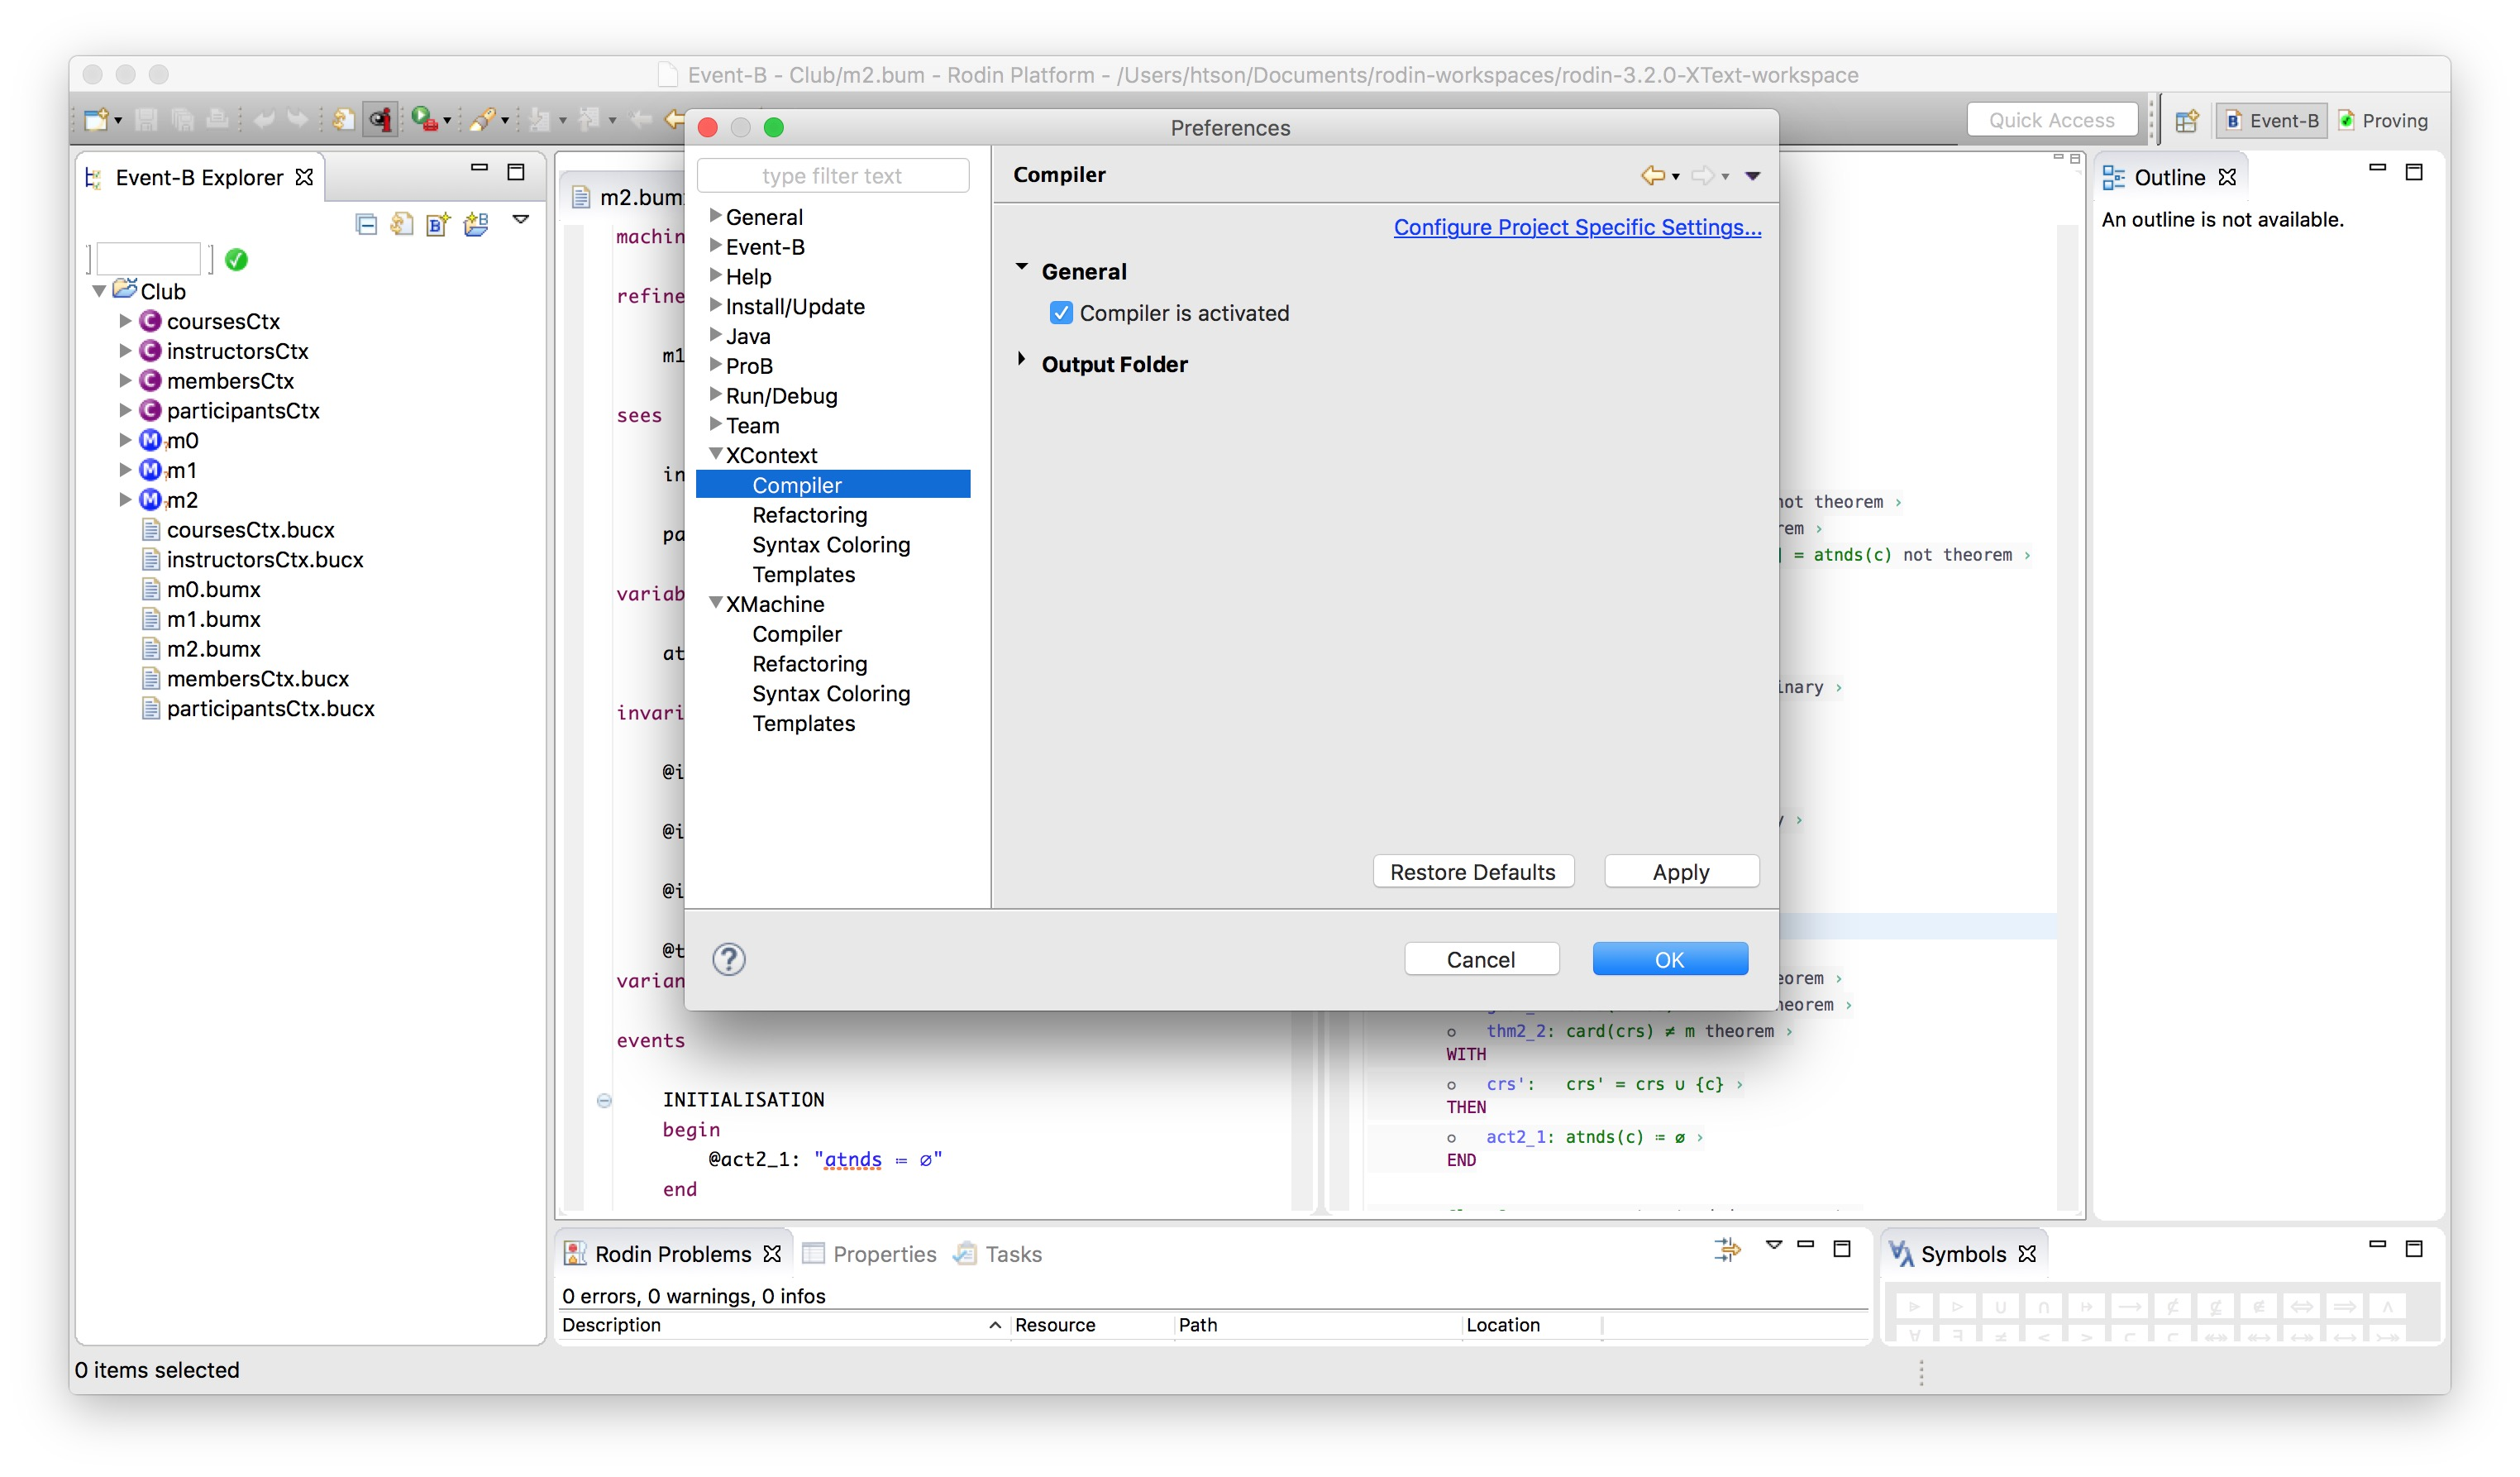
\includegraphics[width=512]{figures/XContextPreference}
%  \else
%  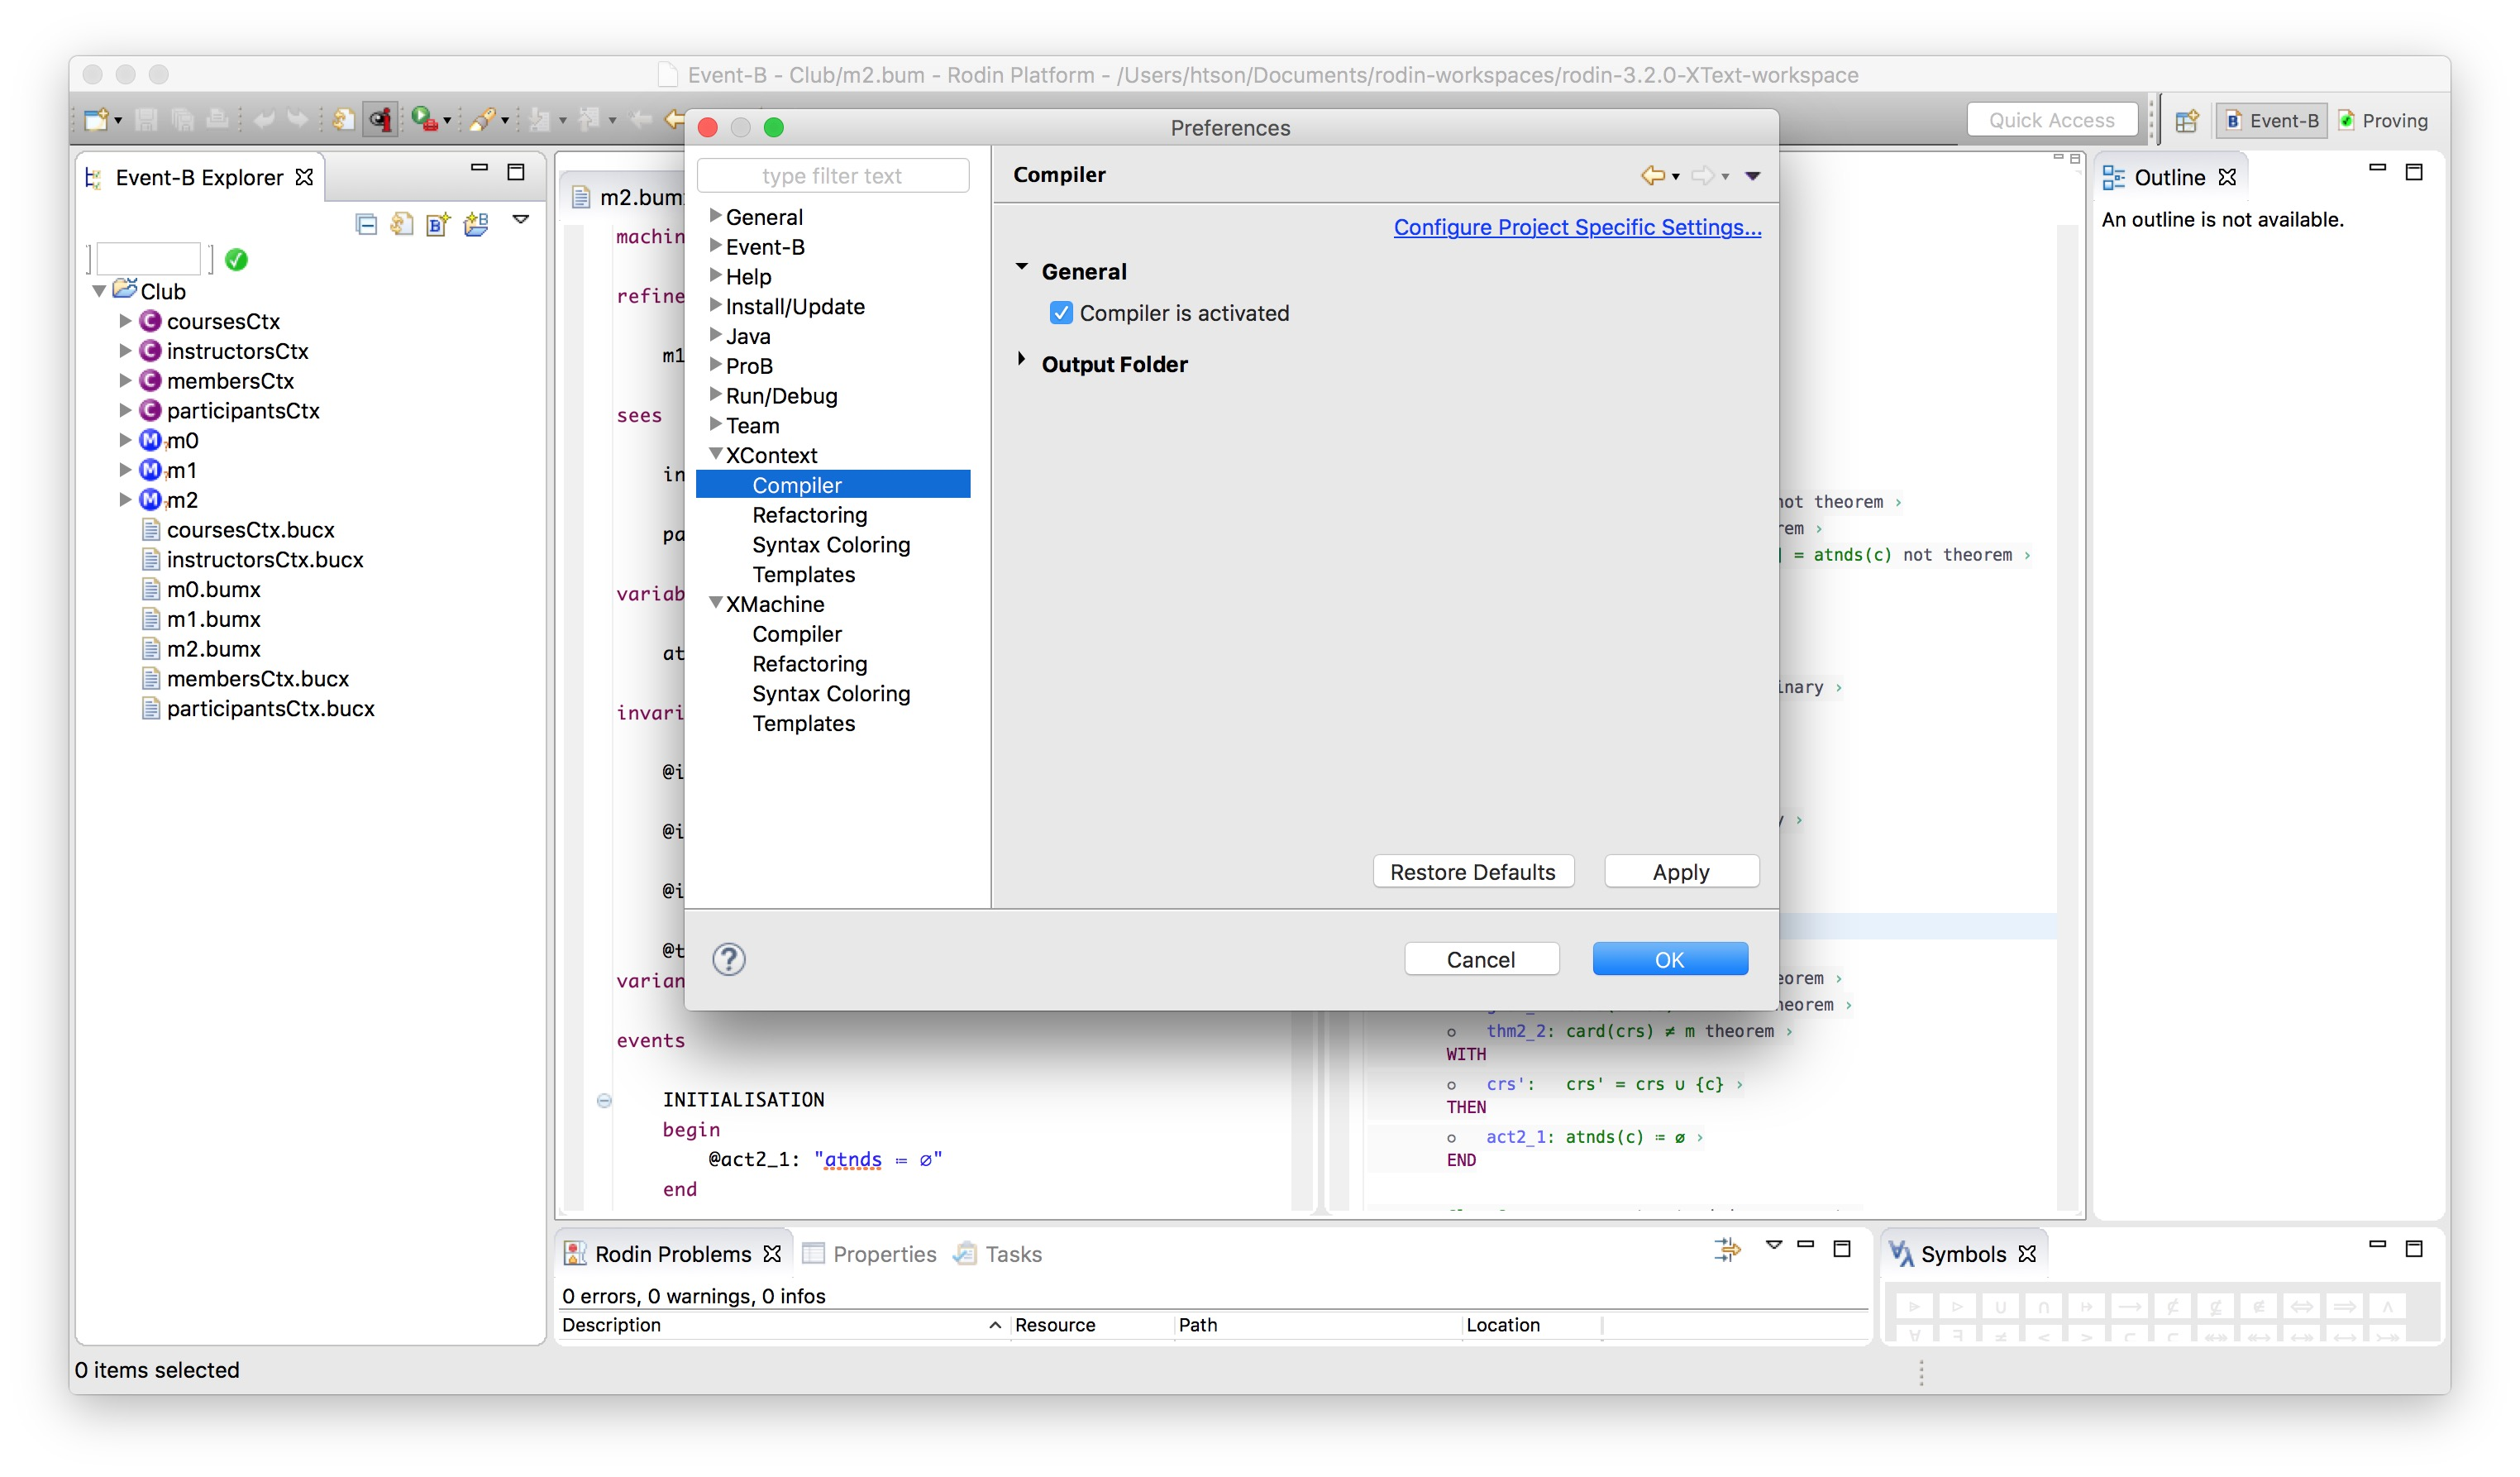
\includegraphics[width=0.9\textwidth]{figures/XContextPreference}
%  \fi
%  \caption{XContext Preference}
%  \label{fig:XContextPreference}
%\end{figure}


%%% Local Variables:
%%% mode: latex
%%% TeX-master: "user_manual"
%%% End:


\section{Tasks}
\label{sec:tasks}

This section is intentionally blank.

%%% Local Variables:
%%% mode: latex
%%% TeX-master: "user_manual"
%%% End:


\section{Reference}
\label{sec:reference}

This section is intentionally blank.

%%% Local Variables:
%%% mode: latex
%%% TeX-master: "user_manual"
%%% End:


%\section{Samples}
\label{sec:samples}


%%% Local Variables:
%%% mode: latex
%%% TeX-master: "user_manual"
%%% End:


\ifplastex
\section{Legal}
\label{sec:legal}

\subsection{EPL Software User Agreement}
\label{sec:user-agreement}


Eclipse Public License - v 1.0

THE ACCOMPANYING PROGRAM IS PROVIDED UNDER THE TERMS OF THIS ECLIPSE PUBLIC LICENSE ("AGREEMENT"). ANY USE, REPRODUCTION OR DISTRIBUTION OF THE PROGRAM CONSTITUTES RECIPIENT'S ACCEPTANCE OF THIS AGREEMENT.

1. DEFINITIONS

"Contribution" means:

a) in the case of the initial Contributor, the initial code and documentation distributed under this Agreement, and
b) in the case of each subsequent Contributor:
i) changes to the Program, and
ii) additions to the Program;
where such changes and/or additions to the Program originate from and are distributed by that particular Contributor. A Contribution 'originates' from a Contributor if it was added to the Program by such Contributor itself or anyone acting on such Contributor's behalf. Contributions do not include additions to the Program which: (i) are separate modules of software distributed in conjunction with the Program under their own license agreement, and (ii) are not derivative works of the Program.
"Contributor" means any person or entity that distributes the Program.

"Licensed Patents " mean patent claims licensable by a Contributor which are necessarily infringed by the use or sale of its Contribution alone or when combined with the Program.

"Program" means the Contributions distributed in accordance with this Agreement.

"Recipient" means anyone who receives the Program under this Agreement, including all Contributors.

2. GRANT OF RIGHTS

a) Subject to the terms of this Agreement, each Contributor hereby grants Recipient a non-exclusive, worldwide, royalty-free copyright license to reproduce, prepare derivative works of, publicly display, publicly perform, distribute and sublicense the Contribution of such Contributor, if any, and such derivative works, in source code and object code form.
b) Subject to the terms of this Agreement, each Contributor hereby grants Recipient a non-exclusive, worldwide, royalty-free patent license under Licensed Patents to make, use, sell, offer to sell, import and otherwise transfer the Contribution of such Contributor, if any, in source code and object code form. This patent license shall apply to the combination of the Contribution and the Program if, at the time the Contribution is added by the Contributor, such addition of the Contribution causes such combination to be covered by the Licensed Patents. The patent license shall not apply to any other combinations which include the Contribution. No hardware per se is licensed hereunder.
c) Recipient understands that although each Contributor grants the licenses to its Contributions set forth herein, no assurances are provided by any Contributor that the Program does not infringe the patent or other intellectual property rights of any other entity. Each Contributor disclaims any liability to Recipient for claims brought by any other entity based on infringement of intellectual property rights or otherwise. As a condition to exercising the rights and licenses granted hereunder, each Recipient hereby assumes sole responsibility to secure any other intellectual property rights needed, if any. For example, if a third party patent license is required to allow Recipient to distribute the Program, it is Recipient's responsibility to acquire that license before distributing the Program.
d) Each Contributor represents that to its knowledge it has sufficient copyright rights in its Contribution, if any, to grant the copyright license set forth in this Agreement.
3. REQUIREMENTS

A Contributor may choose to distribute the Program in object code form under its own license agreement, provided that:

a) it complies with the terms and conditions of this Agreement; and
b) its license agreement:
i) effectively disclaims on behalf of all Contributors all warranties and conditions, express and implied, including warranties or conditions of title and non-infringement, and implied warranties or conditions of merchantability and fitness for a particular purpose;
ii) effectively excludes on behalf of all Contributors all liability for damages, including direct, indirect, special, incidental and consequential damages, such as lost profits;
iii) states that any provisions which differ from this Agreement are offered by that Contributor alone and not by any other party; and
iv) states that source code for the Program is available from such Contributor, and informs licensees how to obtain it in a reasonable manner on or through a medium customarily used for software exchange.
When the Program is made available in source code form:

a) it must be made available under this Agreement; and
b) a copy of this Agreement must be included with each copy of the Program.
Contributors may not remove or alter any copyright notices contained within the Program.

Each Contributor must identify itself as the originator of its Contribution, if any, in a manner that reasonably allows subsequent Recipients to identify the originator of the Contribution.

4. COMMERCIAL DISTRIBUTION

Commercial distributors of software may accept certain responsibilities with respect to end users, business partners and the like. While this license is intended to facilitate the commercial use of the Program, the Contributor who includes the Program in a commercial product offering should do so in a manner which does not create potential liability for other Contributors. Therefore, if a Contributor includes the Program in a commercial product offering, such Contributor ("Commercial Contributor") hereby agrees to defend and indemnify every other Contributor ("Indemnified Contributor") against any losses, damages and costs (collectively "Losses") arising from claims, lawsuits and other legal actions brought by a third party against the Indemnified Contributor to the extent caused by the acts or omissions of such Commercial Contributor in connection with its distribution of the Program in a commercial product offering. The obligations in this section do not apply to any claims or Losses relating to any actual or alleged intellectual property infringement. In order to qualify, an Indemnified Contributor must: a) promptly notify the Commercial Contributor in writing of such claim, and b) allow the Commercial Contributor to control, and cooperate with the Commercial Contributor in, the defense and any related settlement negotiations. The Indemnified Contributor may participate in any such claim at its own expense.

For example, a Contributor might include the Program in a commercial product offering, Product X. That Contributor is then a Commercial Contributor. If that Commercial Contributor then makes performance claims, or offers warranties related to Product X, those performance claims and warranties are such Commercial Contributor's responsibility alone. Under this section, the Commercial Contributor would have to defend claims against the other Contributors related to those performance claims and warranties, and if a court requires any other Contributor to pay any damages as a result, the Commercial Contributor must pay those damages.

5. NO WARRANTY

EXCEPT AS EXPRESSLY SET FORTH IN THIS AGREEMENT, THE PROGRAM IS PROVIDED ON AN "AS IS" BASIS, WITHOUT WARRANTIES OR CONDITIONS OF ANY KIND, EITHER EXPRESS OR IMPLIED INCLUDING, WITHOUT LIMITATION, ANY WARRANTIES OR CONDITIONS OF TITLE, NON-INFRINGEMENT, MERCHANTABILITY OR FITNESS FOR A PARTICULAR PURPOSE. Each Recipient is solely responsible for determining the appropriateness of using and distributing the Program and assumes all risks associated with its exercise of rights under this Agreement , including but not limited to the risks and costs of program errors, compliance with applicable laws, damage to or loss of data, programs or equipment, and unavailability or interruption of operations.

6. DISCLAIMER OF LIABILITY

EXCEPT AS EXPRESSLY SET FORTH IN THIS AGREEMENT, NEITHER RECIPIENT NOR ANY CONTRIBUTORS SHALL HAVE ANY LIABILITY FOR ANY DIRECT, INDIRECT, INCIDENTAL, SPECIAL, EXEMPLARY, OR CONSEQUENTIAL DAMAGES (INCLUDING WITHOUT LIMITATION LOST PROFITS), HOWEVER CAUSED AND ON ANY THEORY OF LIABILITY, WHETHER IN CONTRACT, STRICT LIABILITY, OR TORT (INCLUDING NEGLIGENCE OR OTHERWISE) ARISING IN ANY WAY OUT OF THE USE OR DISTRIBUTION OF THE PROGRAM OR THE EXERCISE OF ANY RIGHTS GRANTED HEREUNDER, EVEN IF ADVISED OF THE POSSIBILITY OF SUCH DAMAGES.

7. GENERAL

If any provision of this Agreement is invalid or unenforceable under applicable law, it shall not affect the validity or enforceability of the remainder of the terms of this Agreement, and without further action by the parties hereto, such provision shall be reformed to the minimum extent necessary to make such provision valid and enforceable.

If Recipient institutes patent litigation against any entity (including a cross-claim or counterclaim in a lawsuit) alleging that the Program itself (excluding combinations of the Program with other software or hardware) infringes such Recipient's patent(s), then such Recipient's rights granted under Section 2(b) shall terminate as of the date such litigation is filed.

All Recipient's rights under this Agreement shall terminate if it fails to comply with any of the material terms or conditions of this Agreement and does not cure such failure in a reasonable period of time after becoming aware of such noncompliance. If all Recipient's rights under this Agreement terminate, Recipient agrees to cease use and distribution of the Program as soon as reasonably practicable. However, Recipient's obligations under this Agreement and any licenses granted by Recipient relating to the Program shall continue and survive.

Everyone is permitted to copy and distribute copies of this Agreement, but in order to avoid inconsistency the Agreement is copyrighted and may only be modified in the following manner. The Agreement Steward reserves the right to publish new versions (including revisions) of this Agreement from time to time. No one other than the Agreement Steward has the right to modify this Agreement. The Eclipse Foundation is the initial Agreement Steward. The Eclipse Foundation may assign the responsibility to serve as the Agreement Steward to a suitable separate entity. Each new version of the Agreement will be given a distinguishing version number. The Program (including Contributions) may always be distributed subject to the version of the Agreement under which it was received. In addition, after a new version of the Agreement is published, Contributor may elect to distribute the Program (including its Contributions) under the new version. Except as expressly stated in Sections 2(a) and 2(b) above, Recipient receives no rights or licenses to the intellectual property of any Contributor under this Agreement, whether expressly, by implication, estoppel or otherwise. All rights in the Program not expressly granted under this Agreement are reserved.

This Agreement is governed by the laws of the State of New York and the intellectual property laws of the United States of America. No party to this Agreement will bring a legal action under this Agreement more than one year after the cause of action arose. Each party waives its rights to a jury trial in any resulting litigation.


%%% Local Variables:
%%% mode: latex
%%% TeX-master: "user_manual"
%%% End:

\else
  \ifstandalone
  \section{Legal}
  \label{sec:legal}

  \subsection{EPL Software User Agreement}
  \label{sec:user-agreement}

  
Eclipse Public License - v 1.0

THE ACCOMPANYING PROGRAM IS PROVIDED UNDER THE TERMS OF THIS ECLIPSE PUBLIC LICENSE ("AGREEMENT"). ANY USE, REPRODUCTION OR DISTRIBUTION OF THE PROGRAM CONSTITUTES RECIPIENT'S ACCEPTANCE OF THIS AGREEMENT.

1. DEFINITIONS

"Contribution" means:

a) in the case of the initial Contributor, the initial code and documentation distributed under this Agreement, and
b) in the case of each subsequent Contributor:
i) changes to the Program, and
ii) additions to the Program;
where such changes and/or additions to the Program originate from and are distributed by that particular Contributor. A Contribution 'originates' from a Contributor if it was added to the Program by such Contributor itself or anyone acting on such Contributor's behalf. Contributions do not include additions to the Program which: (i) are separate modules of software distributed in conjunction with the Program under their own license agreement, and (ii) are not derivative works of the Program.
"Contributor" means any person or entity that distributes the Program.

"Licensed Patents " mean patent claims licensable by a Contributor which are necessarily infringed by the use or sale of its Contribution alone or when combined with the Program.

"Program" means the Contributions distributed in accordance with this Agreement.

"Recipient" means anyone who receives the Program under this Agreement, including all Contributors.

2. GRANT OF RIGHTS

a) Subject to the terms of this Agreement, each Contributor hereby grants Recipient a non-exclusive, worldwide, royalty-free copyright license to reproduce, prepare derivative works of, publicly display, publicly perform, distribute and sublicense the Contribution of such Contributor, if any, and such derivative works, in source code and object code form.
b) Subject to the terms of this Agreement, each Contributor hereby grants Recipient a non-exclusive, worldwide, royalty-free patent license under Licensed Patents to make, use, sell, offer to sell, import and otherwise transfer the Contribution of such Contributor, if any, in source code and object code form. This patent license shall apply to the combination of the Contribution and the Program if, at the time the Contribution is added by the Contributor, such addition of the Contribution causes such combination to be covered by the Licensed Patents. The patent license shall not apply to any other combinations which include the Contribution. No hardware per se is licensed hereunder.
c) Recipient understands that although each Contributor grants the licenses to its Contributions set forth herein, no assurances are provided by any Contributor that the Program does not infringe the patent or other intellectual property rights of any other entity. Each Contributor disclaims any liability to Recipient for claims brought by any other entity based on infringement of intellectual property rights or otherwise. As a condition to exercising the rights and licenses granted hereunder, each Recipient hereby assumes sole responsibility to secure any other intellectual property rights needed, if any. For example, if a third party patent license is required to allow Recipient to distribute the Program, it is Recipient's responsibility to acquire that license before distributing the Program.
d) Each Contributor represents that to its knowledge it has sufficient copyright rights in its Contribution, if any, to grant the copyright license set forth in this Agreement.
3. REQUIREMENTS

A Contributor may choose to distribute the Program in object code form under its own license agreement, provided that:

a) it complies with the terms and conditions of this Agreement; and
b) its license agreement:
i) effectively disclaims on behalf of all Contributors all warranties and conditions, express and implied, including warranties or conditions of title and non-infringement, and implied warranties or conditions of merchantability and fitness for a particular purpose;
ii) effectively excludes on behalf of all Contributors all liability for damages, including direct, indirect, special, incidental and consequential damages, such as lost profits;
iii) states that any provisions which differ from this Agreement are offered by that Contributor alone and not by any other party; and
iv) states that source code for the Program is available from such Contributor, and informs licensees how to obtain it in a reasonable manner on or through a medium customarily used for software exchange.
When the Program is made available in source code form:

a) it must be made available under this Agreement; and
b) a copy of this Agreement must be included with each copy of the Program.
Contributors may not remove or alter any copyright notices contained within the Program.

Each Contributor must identify itself as the originator of its Contribution, if any, in a manner that reasonably allows subsequent Recipients to identify the originator of the Contribution.

4. COMMERCIAL DISTRIBUTION

Commercial distributors of software may accept certain responsibilities with respect to end users, business partners and the like. While this license is intended to facilitate the commercial use of the Program, the Contributor who includes the Program in a commercial product offering should do so in a manner which does not create potential liability for other Contributors. Therefore, if a Contributor includes the Program in a commercial product offering, such Contributor ("Commercial Contributor") hereby agrees to defend and indemnify every other Contributor ("Indemnified Contributor") against any losses, damages and costs (collectively "Losses") arising from claims, lawsuits and other legal actions brought by a third party against the Indemnified Contributor to the extent caused by the acts or omissions of such Commercial Contributor in connection with its distribution of the Program in a commercial product offering. The obligations in this section do not apply to any claims or Losses relating to any actual or alleged intellectual property infringement. In order to qualify, an Indemnified Contributor must: a) promptly notify the Commercial Contributor in writing of such claim, and b) allow the Commercial Contributor to control, and cooperate with the Commercial Contributor in, the defense and any related settlement negotiations. The Indemnified Contributor may participate in any such claim at its own expense.

For example, a Contributor might include the Program in a commercial product offering, Product X. That Contributor is then a Commercial Contributor. If that Commercial Contributor then makes performance claims, or offers warranties related to Product X, those performance claims and warranties are such Commercial Contributor's responsibility alone. Under this section, the Commercial Contributor would have to defend claims against the other Contributors related to those performance claims and warranties, and if a court requires any other Contributor to pay any damages as a result, the Commercial Contributor must pay those damages.

5. NO WARRANTY

EXCEPT AS EXPRESSLY SET FORTH IN THIS AGREEMENT, THE PROGRAM IS PROVIDED ON AN "AS IS" BASIS, WITHOUT WARRANTIES OR CONDITIONS OF ANY KIND, EITHER EXPRESS OR IMPLIED INCLUDING, WITHOUT LIMITATION, ANY WARRANTIES OR CONDITIONS OF TITLE, NON-INFRINGEMENT, MERCHANTABILITY OR FITNESS FOR A PARTICULAR PURPOSE. Each Recipient is solely responsible for determining the appropriateness of using and distributing the Program and assumes all risks associated with its exercise of rights under this Agreement , including but not limited to the risks and costs of program errors, compliance with applicable laws, damage to or loss of data, programs or equipment, and unavailability or interruption of operations.

6. DISCLAIMER OF LIABILITY

EXCEPT AS EXPRESSLY SET FORTH IN THIS AGREEMENT, NEITHER RECIPIENT NOR ANY CONTRIBUTORS SHALL HAVE ANY LIABILITY FOR ANY DIRECT, INDIRECT, INCIDENTAL, SPECIAL, EXEMPLARY, OR CONSEQUENTIAL DAMAGES (INCLUDING WITHOUT LIMITATION LOST PROFITS), HOWEVER CAUSED AND ON ANY THEORY OF LIABILITY, WHETHER IN CONTRACT, STRICT LIABILITY, OR TORT (INCLUDING NEGLIGENCE OR OTHERWISE) ARISING IN ANY WAY OUT OF THE USE OR DISTRIBUTION OF THE PROGRAM OR THE EXERCISE OF ANY RIGHTS GRANTED HEREUNDER, EVEN IF ADVISED OF THE POSSIBILITY OF SUCH DAMAGES.

7. GENERAL

If any provision of this Agreement is invalid or unenforceable under applicable law, it shall not affect the validity or enforceability of the remainder of the terms of this Agreement, and without further action by the parties hereto, such provision shall be reformed to the minimum extent necessary to make such provision valid and enforceable.

If Recipient institutes patent litigation against any entity (including a cross-claim or counterclaim in a lawsuit) alleging that the Program itself (excluding combinations of the Program with other software or hardware) infringes such Recipient's patent(s), then such Recipient's rights granted under Section 2(b) shall terminate as of the date such litigation is filed.

All Recipient's rights under this Agreement shall terminate if it fails to comply with any of the material terms or conditions of this Agreement and does not cure such failure in a reasonable period of time after becoming aware of such noncompliance. If all Recipient's rights under this Agreement terminate, Recipient agrees to cease use and distribution of the Program as soon as reasonably practicable. However, Recipient's obligations under this Agreement and any licenses granted by Recipient relating to the Program shall continue and survive.

Everyone is permitted to copy and distribute copies of this Agreement, but in order to avoid inconsistency the Agreement is copyrighted and may only be modified in the following manner. The Agreement Steward reserves the right to publish new versions (including revisions) of this Agreement from time to time. No one other than the Agreement Steward has the right to modify this Agreement. The Eclipse Foundation is the initial Agreement Steward. The Eclipse Foundation may assign the responsibility to serve as the Agreement Steward to a suitable separate entity. Each new version of the Agreement will be given a distinguishing version number. The Program (including Contributions) may always be distributed subject to the version of the Agreement under which it was received. In addition, after a new version of the Agreement is published, Contributor may elect to distribute the Program (including its Contributions) under the new version. Except as expressly stated in Sections 2(a) and 2(b) above, Recipient receives no rights or licenses to the intellectual property of any Contributor under this Agreement, whether expressly, by implication, estoppel or otherwise. All rights in the Program not expressly granted under this Agreement are reserved.

This Agreement is governed by the laws of the State of New York and the intellectual property laws of the United States of America. No party to this Agreement will bring a legal action under this Agreement more than one year after the cause of action arose. Each party waives its rights to a jury trial in any resulting litigation.


%%% Local Variables:
%%% mode: latex
%%% TeX-master: "user_manual"
%%% End:

  \else
  \fi
\fi

%%% Local Variables:
%%% mode: latex
%%% TeX-master: "user_manual"
%%% End:


\end{document}

%%% Local Variables:
%%% mode: latex
%%% TeX-master: t
%%% End:
